\documentclass[french]{article}
\usepackage{aeguill,aecompl,babel,tikz,geometry}
\usetikzlibrary{arrows} % package de flèches
\usepackage[T1]{fontenc}
\usepackage[utf8]{inputenc}
\pagestyle{empty}
\geometry{
paperwidth=22cm,
paperheight = 14.5cm,
left=0pt,
right=0pt,
top=2pt,
bottom=0pt
}
%\tikzset{%
%cat/.style={right=2cm,anchor=west,align=left},
%subcat/.style={below=1cm,anchor=north west,draw=none,font=\em,align=left}
%}
%\pgfdeclarelayer{background}
%\pgfsetlayers{background,main}

\begin{document}
\centering

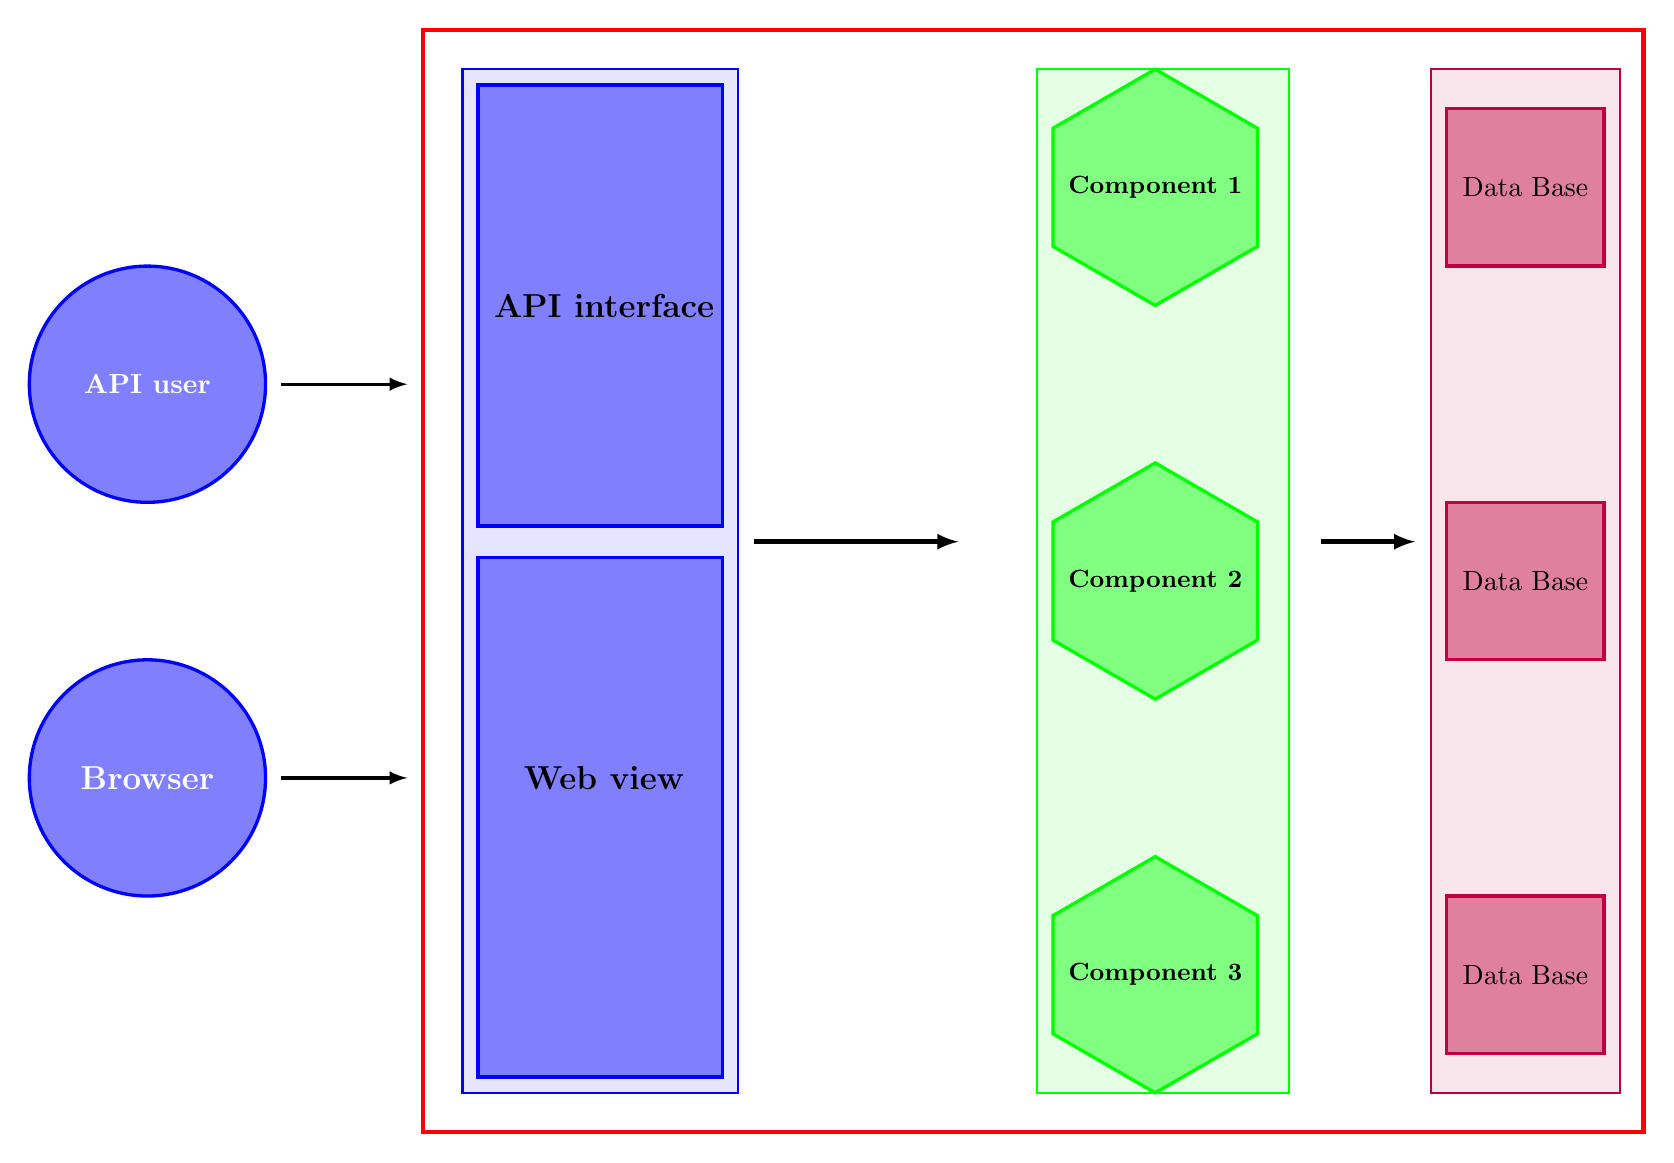
\begin{tikzpicture}

\draw [blue,fill=blue!50, very thick] (1.5,4) circle (1.5);
\draw (1.5,4) node[white] {\large{\textbf{Browser}}};
\draw [very thick, >=latex, ->] (3.2,4) -- (4.8,4);

\draw [blue,fill=blue!50, very thick] (1.5,9) circle (1.5);
\draw (1.5,9) node[white] {\textbf{API user}};
\draw [very thick, >=latex, ->] (3.2,9) -- (4.8,9);

\draw [red, ultra thick] (5,13.5) rectangle (20.5,-0.5);

\draw [blue,fill=blue!10, thick] (5.5,13) rectangle (9,0);
\draw [blue,fill=blue!50, very thick] (5.7,6.8) rectangle (8.8,0.2);
\draw (7.3,4) node {\large{\textbf{Web view}}};
\draw [blue,fill=blue!50, very thick] (5.7,12.8) rectangle (8.8,7.2);
\draw (7.3,10) node {\large{\textbf{API interface}}};
\draw [ultra thick, >=latex, ->] (9.2,7) -- (11.8,7);

\draw [green,fill=green!10, thick] (12.8,13) rectangle (16,0);
\draw [green,fill=green!50, very thick] (13,12.25) -- (13,10.75)
-- ++(-30:1.5) -- ++(30:1.5) -- ++(90:1.5) -- ++(150:1.5) -- cycle;
\draw (14.3,11.5) node {\small{\textbf{Component 1}}};
\draw [green,fill=green!50, very thick] (13,7.25) -- (13,5.75)
-- ++(-30:1.5) -- ++(30:1.5) -- ++(90:1.5) -- ++(150:1.5) -- cycle;
\draw (14.3,6.5) node {\small{\textbf{Component 2}}};
\draw [green,fill=green!50, very thick] (13,2.25) -- (13,0.75)
-- ++(-30:1.5) -- ++(30:1.5) -- ++(90:1.5) -- ++(150:1.5) -- cycle;
\draw (14.3,1.5) node {\small{\textbf{Component 3}}};
\draw [ultra thick, >=latex, ->] (16.4,7) -- (17.6,7);

\draw [purple,fill=purple!10, thick] (17.8,13) rectangle (20.2,0);
\draw [purple,fill=purple!50, very thick] (18,12.5) rectangle (20,10.5);
\draw (19,11.5) node {Data Base};
\draw [purple,fill=purple!50, very thick] (18,7.5) rectangle (20,5.5);
\draw (19,6.5) node {Data Base};
\draw [purple,fill=purple!50, very thick] (18,2.5) rectangle (20,0.5);
\draw (19,1.5) node {Data Base};

\end{tikzpicture}

\end{document}
